\begin{center}
  \setstretch{1.0}
  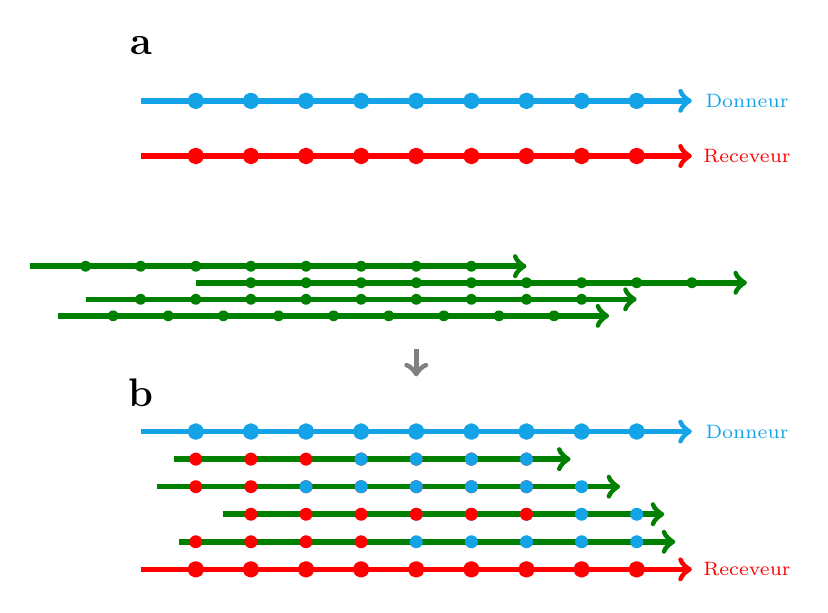
\begin{tikzpicture}[scale=0.7, line width = 2pt, join=round]

    \tikzstyle{every node}=[font=\scriptsize]

    %% ref align
    \begin{scope}[shift={(0, 17.5)}]
      \draw[Black] (0, 2) node {\Large \bfseries a};

      \draw[Red] [->] (0, 0) -- (10, 0);
      \draw[Cerulean] [->] (0, 1) -- (10, 1);

      \foreach \x in {1,2,...,9}
      {
        \draw[color = Red, fill = Red] (\x, 0) circle (0.1);
        \draw[color = Cerulean, fill = Cerulean] (\x, 1) circle (0.1);
      }

      \draw[Red] (11, 0) node {Receveur};
      \draw[Cerulean] (11, 1) node {Donneur};

      \draw[Green] [->] (-2, -2) -- (7, -2);
      \draw[Green] [->] (1, -2.3) -- (11, -2.3);
      \draw[Green] [->] (-1, -2.6) -- (9, -2.6);
      \draw[Green] [->] (-1.5, -2.9) -- (8.5, -2.9);

      \foreach \x in {-1,0,...,6} { \draw[color = Green, fill = Green] (\x, -2)   circle (0.05);  }
      \foreach \x in {2,3,...,10} { \draw[color = Green, fill = Green] (\x, -2.3) circle (0.05);  }
      \foreach \x in {0,1,...,8 } { \draw[color = Green, fill = Green] (\x, -2.6) circle (0.05);  }
      \foreach \x in {-0.5,0.5,...,7.5 } { \draw[color = Green, fill = Green] (\x, -2.9) circle (0.05);  }

      \draw[Gray] [->] (5, -3.5) -- (5, -4);
    \end{scope}

    \begin{scope}[shift={(0, 10)}]
      %% align reads to reference
      \draw[Black] (0, 3.2) node {\Large \bfseries b};

      \draw[Red] (11, 0) node {Receveur};
      \draw[Cerulean] (11, 2.5) node {Donneur};

      \draw[Red] [->] (0, 0) -- (10, 0);
      \draw[Cerulean] [->] (0, 2.5) -- (10, 2.5);

      \foreach \x in {1,2,...,9}
      {
        \draw[color = Red, fill = Red] (\x, 0) circle (0.1);
        \draw[color = Cerulean, fill = Cerulean] (\x, 2.5) circle (0.1);
      }

      \draw[Green] [->] (0.7, 0.5) -- (9.7, 0.5);
      \foreach \x in {5,6,...,9} { \draw[color = Cerulean, fill = Cerulean] (\x, 0.5)   circle (0.07);  }
      \foreach \x in {1,2,...,4} { \draw[color = Red, fill = Red] (\x, 0.5)   circle (0.07);  }
      \draw[Green] [->] (1.5, 1) -- (9.5, 1);
      \foreach \x in {5,6,...,9} { \draw[color = Cerulean, fill = Cerulean] (\x, 1.0)   circle (0.07);  }
      \foreach \x in {2,3,...,7} { \draw[color = Red, fill = Red] (\x, 1.0)   circle (0.07);  }
      \draw[Green] [->] (0.3, 1.5) -- (8.7, 1.5);
      \foreach \x in {1,2,...,7} { \draw[color = Red, fill = Red] (\x, 1.5)   circle (0.07);  }
      \foreach \x in {3,4,...,8} { \draw[color = Cerulean, fill = Cerulean] (\x, 1.5)   circle (0.07);  }
      \draw[Green] [->] (0.6, 2.0) -- (7.8, 2.0);
      \foreach \x in {1,2,...,7} { \draw[color = Red, fill = Red] (\x, 2.0)   circle (0.07);  }
      \foreach \x in {4,5,...,7} { \draw[color = Cerulean, fill = Cerulean] (\x, 2.0)   circle (0.07);  }
    \end{scope}


  \end{tikzpicture}
\end{center}
